\chapter{Probabilistic TFA of \textit{C. elegans}}\label{ch:Probabilistic_TFA}

% **************************** Define Graphics Path **************************
\ifpdf
    \graphicspath{{Chapter2/Figs/Raster/}{Chapter2/Figs/PDF/}{Chapter2/Figs/}}
\else
    \graphicspath{{Chapter2/Figs/Vector/}{Chapter2/Figs/}}
\fi

The data – information – knowledge – wisdom (DIKW) hierarchy is one of the fundamental and widely recognized hierarchy in the information and knowledge literature. This hierarchy contextualize data, information, knowledge, and wisdom, with respect to one another to identify and describe the processes involved in the transformation of lower level entity of the hierarchy to a higher level one (\cite{Rowley:2007}). The increasing availability of very high dimensional data with diverse characteristics and growing complexity playing the vital role behind the recent advancement of machine learning techniques. Figure \ref{fig:High_dimensional_data} shows some example of high-dimensional data from different domains, types and nature.
 
Data from real world likely to suffer from quality issue for various reasons. Even in the controlled environment due to several reasons acquisition errors might be included. In the noisy environment it might be even more. Dealing with these noise or added uncertainty of the data is troublesome. In a particular context within the constraints probabilistic modelling turns out to be a dominant approach with added flexibility and capability of dealing with uncertainty in many forms.

\begin{figure}
	\centering
		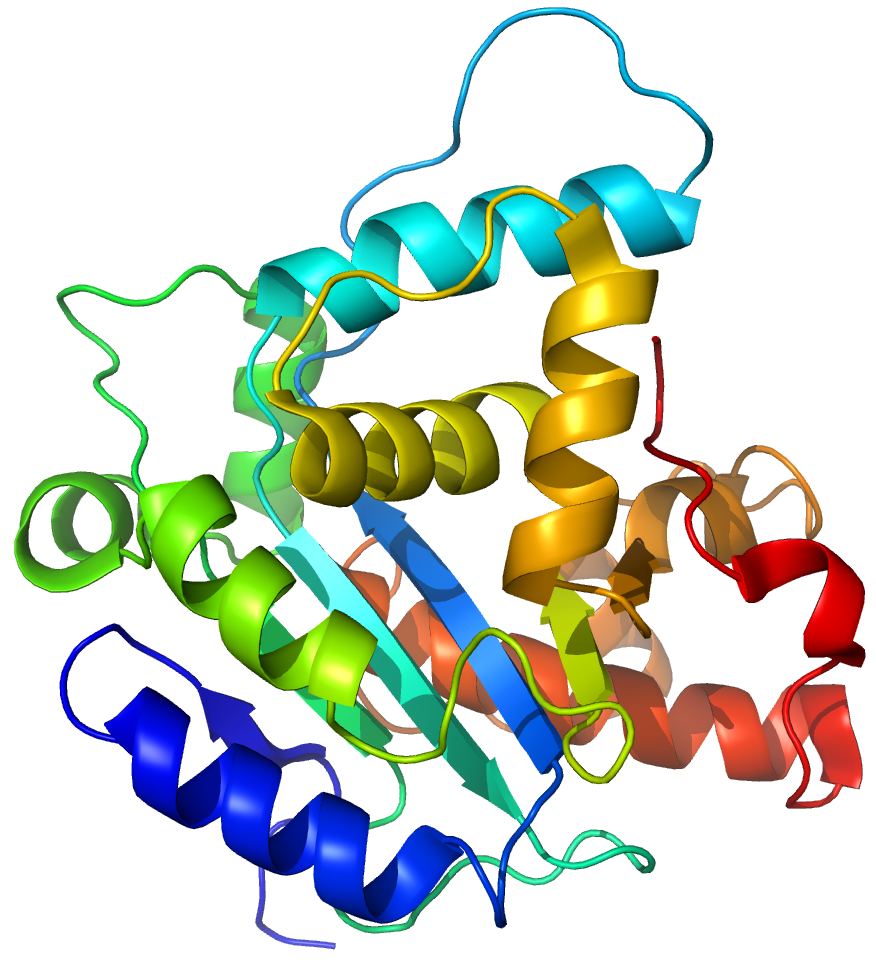
\includegraphics[width=0.27\textwidth,keepaspectratio]{protein_structure4.png}
		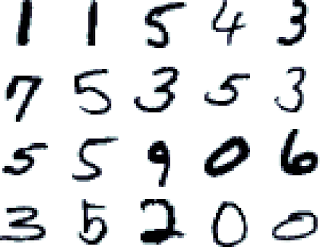
\includegraphics[width=0.3\textwidth,keepaspectratio]{mnist.png}
		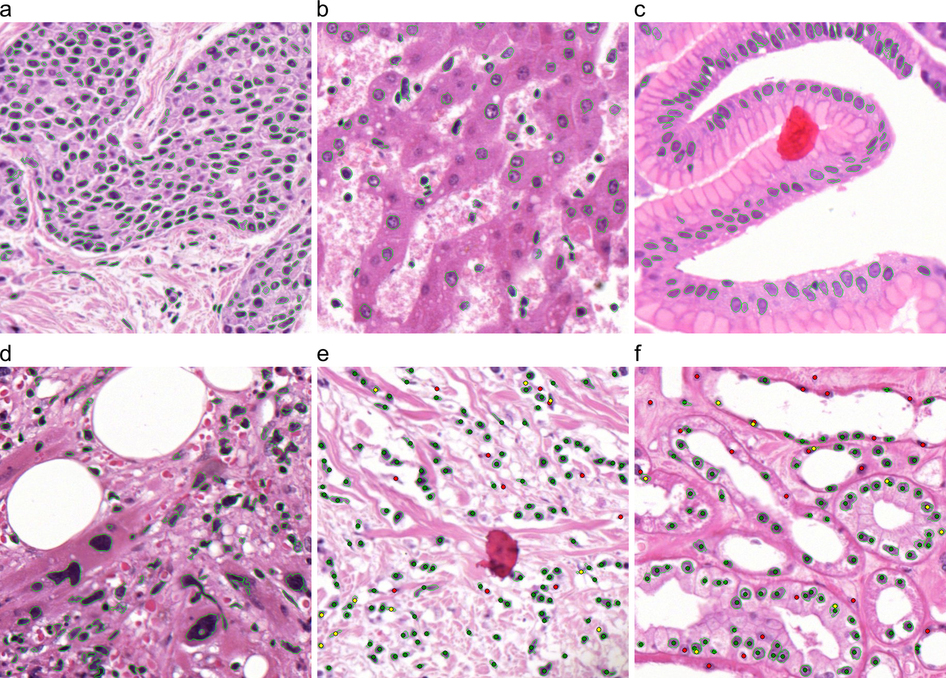
\includegraphics[width=0.35\textwidth,keepaspectratio]{srep00503-f1.jpg}
		\rule{35em}{0.5pt}
	\caption[Examples of high dimensional data form types and nature]
		{Examples of high dimensional data form types and nature. Left: 3D model of a 
		protein structure. Centre: Multiple
		samples of hand written digits from MNIST dataset. available at 
		\url{http://yann.lecun.com/exdb/mnist/}. Right: Multiple image patch 
		from breast cancer, liver, gastric mucosa, bone marrow connective tissue, kidney tissue for 
		virtual microscopy (\cite{Wienert:2012}) }
	\label{fig:High_dimensional_data}
\end{figure}

\section{Latent Variable Model}
Latent variable models (LVMs) (\cite{Bishop:1999}) explain complex relations between multiple variables by simple relations between the variables and an underlying unobservable, i.e. latent structure. Latent variable are typically included in statistical model for different statistical concepts, including representation the unobservable factors/covariates, missing data, random effects, finite mixtures, variations in hierarchical data, and clusters and many more. Figure \ref{fig:LVM Cartton} shows an analogy of latent variable model where Marionette's different movement and dynamics are observed whereas these movements are taking place or controlled by the 'control bar'. The dynamics of the control bar is usually unobserved.

A set of latent (or hidden, or directly not observable) variables $\textbf{X}$ that can be related to the observed variables $\textbf{Y}$ defines by a joint distribution over both. The latent space is 
controlled by a prior distribution $p\left(\textbf{X}\right)$ over the distribution of $\textbf{Y}$ under the assumption of a probabilistic mapping of the form
\begin{equation} \label{eq:linear_model}
y_{i,j} = f_j\left(\textbf{x}_{i}\right) + \epsilon_{i},
\end{equation}
where $\textbf{x}_i \in \mathbb{R}^q$ is the latent point associated with the $i^{th}$ observation $\textbf{y}_i \in \mathbb{R}^p$, $j$ is the index of the features of $\textbf{Y}$. Inaccuracy of
the model  and the noise of the data is modelled by the additional noise parameter $\epsilon_{i}$. Typically it is assumed that the noise has a Gaussian distribution $\epsilon \sim \mathcal{N} \left(0,\beta^{-1}\right)$, where the term $\beta$ is the precision.

We can map $f$ of Equation \ref{eq:linear_model} as linear and equal to a matrix $\textbf{W}\in\mathbb{R}^{p\times q}$. Then we can rewrite the Equation \ref{eq:linear_model} as
\begin{equation} \label{eq:linear_model_matrix}
y_{i,j} = w_j\left(\textbf{x}_{i}\right) + \epsilon_{i},
\end{equation}
where $w_j$ are the rows of $\textbf{W}$. This model is known as probabilistic version of principal component analysis (PPCA) (\cite{Roweis:1998, Tipping:1999}). 

\begin{figure}
	\centering
		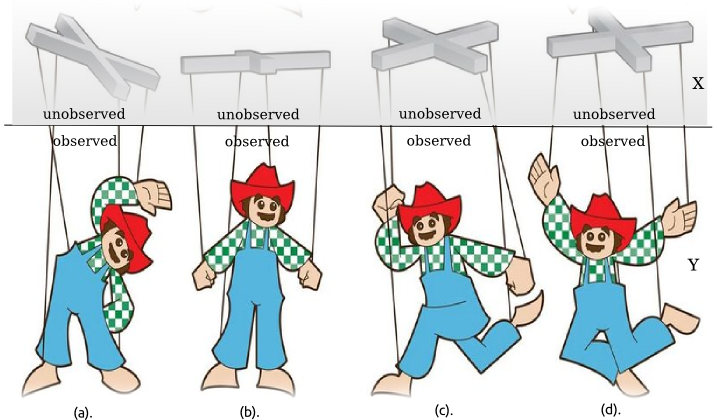
\includegraphics[width=0.7\textwidth,keepaspectratio]{LVM_Cartoon.png}
		\rule{35em}{0.5pt}
	\caption[Marionette Analogy of Latent Variable Model]
		{Marionette Analogy of Latent Variable Model: Marionette's different dynamics are observed (represented by $\textbf{Y}$). But these movements are controlled by the control bar which is unobserved (dynamics represented by $\textbf{X}$).}
	\label{fig:LVM Cartton}
\end{figure}

Given the prior distribution over the latent variables has a Gaussian distribution, then the precision $\beta$ can be infinity and PCA is recovered in the limit. The conditional probability
of the data given the latent space is:
\begin{equation} \label{eq:cond_prob_latent_space}
p\left(\textbf{y}_i|\textbf{x}_i,\textbf{W},\beta \right) = \mathcal{N} \left(\textbf{y}_i|\textbf{W}\textbf{x}_i,\beta^{-1}\textbf{I}\right).
\end{equation}
If we consider data points are independent, then the marginal likelihood of the data is obtained by:
\begin{equation} \label{eq:marginal_likelihood_latent_space}
p\left(\textbf{Y}|\textbf{W},\beta \right) = 
\int \prod^{N}_{i=1} p\left(\textbf{y}_i|\textbf{x}_i,\textbf{W},\beta\right)p\left(\textbf{x}_i\right)d\textbf{x}.
\end{equation}
Even for finite precision $\beta$ the maximum likelihood solution for $\textbf{W}$ spans the principal sub-space of the data (\cite{Tipping:1999}). This approach is can be applicable for both 
linear (e.g.\ \cite{Silva:2006}) and non-linear (e.g.\ GP-LVM by \cite{Lawrence:2005}) models. The classical approach while dealing with this latent variables is first they are marginalised then
other parameters are optimized using maximum likelihood model. \cite{Lawrence:2005} used an alternative but similar approach by first marginalising the parameters and then optimized the
latent variables.

\section{Modelling of TFAs}
In recent years most methods aim to infer a matrix of transcription factor activities (TFAs). These TFAs are sum up in a single number at a certain experimental point to find the concentration of the transcription factor and its binding affinity to its target genes. Many of the researcher used different ways or algorithm to find out these TFAs. For example, \cite{Liao:2003} developed a data decomposition technique with dimension reduction and introduced ‘network component analysis’. This method takes account of the connectivity information by imposing algebraic constraints on the factors. They argued that classical statistical methods such as principal component analysis and independent component analysis dose not consider the underlying network structure while computing low dimensional or hidden representation of a high-dimensional data sets like DNA microarray. 

\cite{Alter:2004} used a dimension reduction technique (SVD) to figure out TFAs and also the correlation between DNA replication initiation and RNA transcription during the yeast cell cycle. Using multivariate regression and backward variable selection to identify active transcription factors \cite{Gao:2004} targeted the same; \cite{Boulesteix:2005} used partial least squares (PLS) regression to infer the true TFAs from a combination of tRNA expression and DNA protein binding measurement. A major drawback of the above mentioned methods is that transcription factor activities do not hold any information regarding the strength of the regulators interactivity between the transcription factor and its different target genes. But it is expected that depending on the experimental conditions transcription factor activities can vary from gene to gene. Even it is also expected that different transcription factors may bind the same gene. In most of the cases, realistic information about the intervals may not be true as they were not based on fully probabilistic model. Moreover, false positives are always a problem for connectivity data, typically a large portion of Chip data suffers form it (\cite{Boulesteix:2005}). Furthermore, due to the various cellular process or changes in environmental conditions the structure of the regulatory network of the cell can change considerably. Using regression-based methods it is difficult to track these changes. \cite{Nachman:2004} build a probabilistic model, using the basic framework of dynamic Bayesian networks using discrete random variables for protein concentrations and binding affinities. Though the model was more realistic but the computational complexity for genome-wide analysis can be expensive.

\section{Our Goal}
In this chapter we will build a dynamic model that extends the linear regression model of \cite{Liao:2003} and probabilistic model of \cite{Sanguinetti:2006} to model the distribution of each transcription factor acting on each gene for a multicellular eukaryote (\textit{C.elegans}). By nature this model will be a latent variable model which will be developed based on probabilistic approach. We will build a tool using programming language $R$ and it will be available on GitHub\footnote{GitHub is a Web-based repository hosting service and source code management platform.}. At Chapter:\ref{ch:GP_Model_of_TFAs} we will model the temporal changes in the gene-specific TFAs from time-series gene expression data using Gaussian process (a stochastic process whose consciousness comes from random values and where the random variables has a normal distribution and it is associated with every single point in a range of times or of space; Chapter:\ref{ch:GaussianProcessRegression} contains detail explanation). The covariance structure of the transcription factors will be shared among all genes. This approach will lead to a manageable parameter space and figure out useful information about the correlation of TFAs.

\section{Probabilistic TFAs}\label{sec:Probabilistic_TFA}
We have developed our $R$ based tools $chipDyno$ based on the probabilistic approach of \cite{Sanguinetti:2006}. First we will give a brief introduction of that approach then we will present results.

The logged gene expression measurements are collected in a design matrix, $\textbf{Y} \in \mathbb{R}^{ N \times d}$ where $N$ is the number of genes and $d$ the time points or number of experiments. 
The connectivity measurements are collected in a binary matrix $\textbf{X} \in \mathbb{R} ^ {N \times q}$, where $q$ is the number of transcription factors; element $(i, j)$ of $\textbf{X}$ is one 
if transcription factor $j$ can bind gene $i$, zero otherwise.

In \cite{Sanguinetti:2006}, TFAs are obtained by regressing the gene expressions using the connectivity information, giving the following linear model- 
\begin{equation} \label{eq:linear_model_TFA}
\textbf{y}_n = \textbf{B}_n \textbf{x}_n + \boldsymbol{\epsilon_{n}}
\end{equation}
Here $n = 1, . . . ,N$ indexes the gene, $\textbf{y}_n =\textbf{Y}(n,:)^{\top}$, $\textbf{x}_n=\textbf{X}(n,:)^{\top}$ and $\boldsymbol{\epsilon_{n}}$ is an error term. The matrix $\textbf{B}_n$ has $d$ rows and $q$ columns, and models the gene specific TFAs.

Different TFAs for every individual gene will increase number of model parameters drastically. But through marginalization by prior distribution on the rows of $\textbf{B}_n$ these parameters can be dealt. Two plausible assumptions for selecting the prior distribution will be helpful to determine the gene specific TFAs. Firstly, $\textbf{b}_{nt}$ has the Markov property and hence gene specific TFA $\textbf{b}_{nt} $ at time $t$ depends solely on the gene specific TFA at time $(t-1)$ and the second assumption is, the prior distribution to be stationary in time.

To satisfy these conditions then there will be two limiting conditions of prior distributions- Assume all the $\textbf{b}_{nt}$ are identical, then the first limiting case will take place. So that
\begin{equation} \label{eq:limit_one_a}
   \textbf{b}_{n1} \sim \mathcal{N} ( \boldsymbol{\mu},\boldsymbol{\Sigma}), 
\end{equation}
and
\begin{equation} \label{eq:limit_one_b}
   \textbf{b}_{n(t+1)} \sim \mathcal{N} ( \textbf{b}_{nt},\textbf{0})
\end{equation}
If the experimental dataset comes by replicating a condition then this model will be an appropriate model. The second limiting case appears when all the $\textbf{b}_{nt}$ are independent and identically distributed
\begin{equation} \label{eq:limit_two}
   \textbf{b}_{nt}\sim \mathcal{N} ( \boldsymbol{\mu},\boldsymbol{\Sigma})
\end{equation}
This is the case when experimental dataset comes from independent samples drawn without any temporal order.

\cite{Sanguinetti:2006}  expected a realistic model of time series data to be somewhere in between this two extremes (Equation:\ref{eq:limit_one_a}, Equation:\ref{eq:limit_one_b} and Equation:\ref{eq:limit_two})
\begin{equation} \label{eq:tfa_SanG_update}
  \textbf{b}_{n(t+1)} \sim \mathcal{N} (\gamma \textbf{b}_{nt} + (1-\gamma)\boldsymbol{\mu},(1-\gamma^2)\boldsymbol{\Sigma})
\end{equation}
for $ t= 1, ... , (d-1)$ and $ \textbf{b}_{n1} \sim \mathcal{N} ( \boldsymbol{\mu},\boldsymbol{\Sigma})$
where $\gamma$ is a parameter measuring the degree of temporal continuity of the TFAs. If genes are independent for given TFA then the likelihood function is given by
\begin{equation} \label{eq:likelihood_fnc}
  p\left(\textbf{Y}|\textbf{B,X}\right)= \prod_{n \mathop = 1}^{N} p\left(\textbf{y}_n|\textbf{B}_n,\textbf{x}_n\right).
\end{equation}
Considering Gaussian noise $\boldsymbol{\epsilon}_n \sim \mathcal{N} \left(0,\boldsymbol{\sigma}^2\textbf{I}\right)$ we have
\begin{equation} \label{eq:likelihood_fnc_SingleGene}
  p\left(\textbf{y}_n|\textbf{B}_n,\textbf{x}_n\right)= \mathcal{N} \left(\textbf{y}_n|\textbf{B}_n \textbf{x}_n, \boldsymbol{\sigma}^2\textbf{I} \right).
\end{equation}
Factorizing the likelihood along the experiments with the assumption of spherical Gaussian noise distribution we can rewrite the Equation \ref{eq:likelihood_fnc} as
\begin{equation} \label{eq:likelihood_factorize}
  p\left(\textbf{Y}|\textbf{B},\textbf{X}\right)= 
     \prod_{t \mathop = 1}^{d} \prod_{n \mathop = 1}^{N} p\left(\textbf{y}_{nt}|\textbf{b}_{nt},\textbf{x}_n\right)
\end{equation}
where
\begin{equation} \label{eq:likelihood_fnc_allGene}
  p\left(\textbf{y}_{nt}|\textbf{b}_{nt},\textbf{x}_n\right)= \mathcal{N} \left(\textbf{y}_{nt}|\textbf{b}^\top_{nt}\textbf{x}_n,\sigma^2 \right).
\end{equation}
Using the classical approach of latent variable model analysis a marginal likelihood for the observations can be obtained by

\begin{equation} \label{eq:marginal_likelihood_tfa}
\begin{aligned}
p\left(\textbf{y}_n|\sigma,\Sigma,\boldsymbol{\mu},\gamma,\textbf{x}_n\right) = &
\int \prod^{d}_{t=1} d\textbf{b}_{nt}\mathcal{N} \left(\textbf{y}_{nt}|\textbf{b}^\top_{nt}\textbf{x}_n, \sigma^2 \right)\\
& \times \left( \prod^{d}_{t=2} p\left(\textbf{b}_{nt}|\textbf{b}_{n(t-1)}\right) \right)
\mathcal{N} \left(\textbf{b}_{n1}|\boldsymbol{\mu}\Sigma \right).
\end{aligned}
\end{equation}

TFAs can be estimated as a posteriori using Bayes’s Theorem. The detail explanation is available at \cite{Sanguinetti:2006}.
% \begin{equation} \label{eq:Bayes_Theorem}
%   p\left(\textbf{b}_n|\textbf{Y}\right)= \frac {p\left(\textbf{Y|b}_n\right) p\left(\textbf{b}_n\right)}{p\left(\textbf{Y}\right)}
% \end{equation}

%----------------------------------------------------------
%----------------------------------------------------------------------------------------
\section{Datasets}
\cite{Sanguinetti:2006} has done their experiments on yeast's cell cycle data of \cite{Spellman:1998} which is a unicellular microorganism. One of our research key question was can we step forward to find out the transcription factor activities from a unicellular microorganism to multicellular eukaryote. \textit{C. elegans} is a established multicellular eukaryotic model organism (Chapter:\ref{ch:Introduction} contains some introductory information about this model organism). To find out the TFA of \textit{C. elegans} basically we had to work with three type of datasets. $i).$ Gene expression time series data $ii).$ Transcription Factors $iii).$ Connectivity information between genes and transcription factors.

\subsection{Gene Expression Time series data}
The gene expression Affymetrix single colour GeneChip data\footnote{We would like to acknowledge Professor Andrew Cossins, Institute of Integrative Biology, University of Liverpool, UK for providing us the data set with valuable information and also for the permission for further analysis of the data.} on point estimate of expression level came without estimates of uncertainty level. To extract this data we used Bioconductor\footnote{The Bioconductor project is an open source software framework to assist biologists and statisticians working in bioinformatics} package \textit{puma} (\cite{puma}). The experiments were done at five different stages (i.e.\ our experimental dataset will have five time points). Apart from the temperature rest of the environmental conditions were same with the target of consistent result. The experimental data was collected within one day of its adulthood at the temperature $20\,^{\circ}\mathrm{C}$. With the target to measure the gene response to chill exposure the temperature was reduced to $5\,^{\circ}\mathrm{C}$ and samples were collected after one hour, then after 24 hour (1 day), then after 72 hours (3 days). For final experiments the temperature was brought back to $20\,^{\circ}\mathrm{C}$
and samples were collected within one day  of rise of temperature. All the experiments were repeated two more times which provide us 3 independent replicates of similar experiments. Figure \ref{fig:PCA_time_series} shows the PCA analysis of the time series data.


\begin{figure}
	\centering
		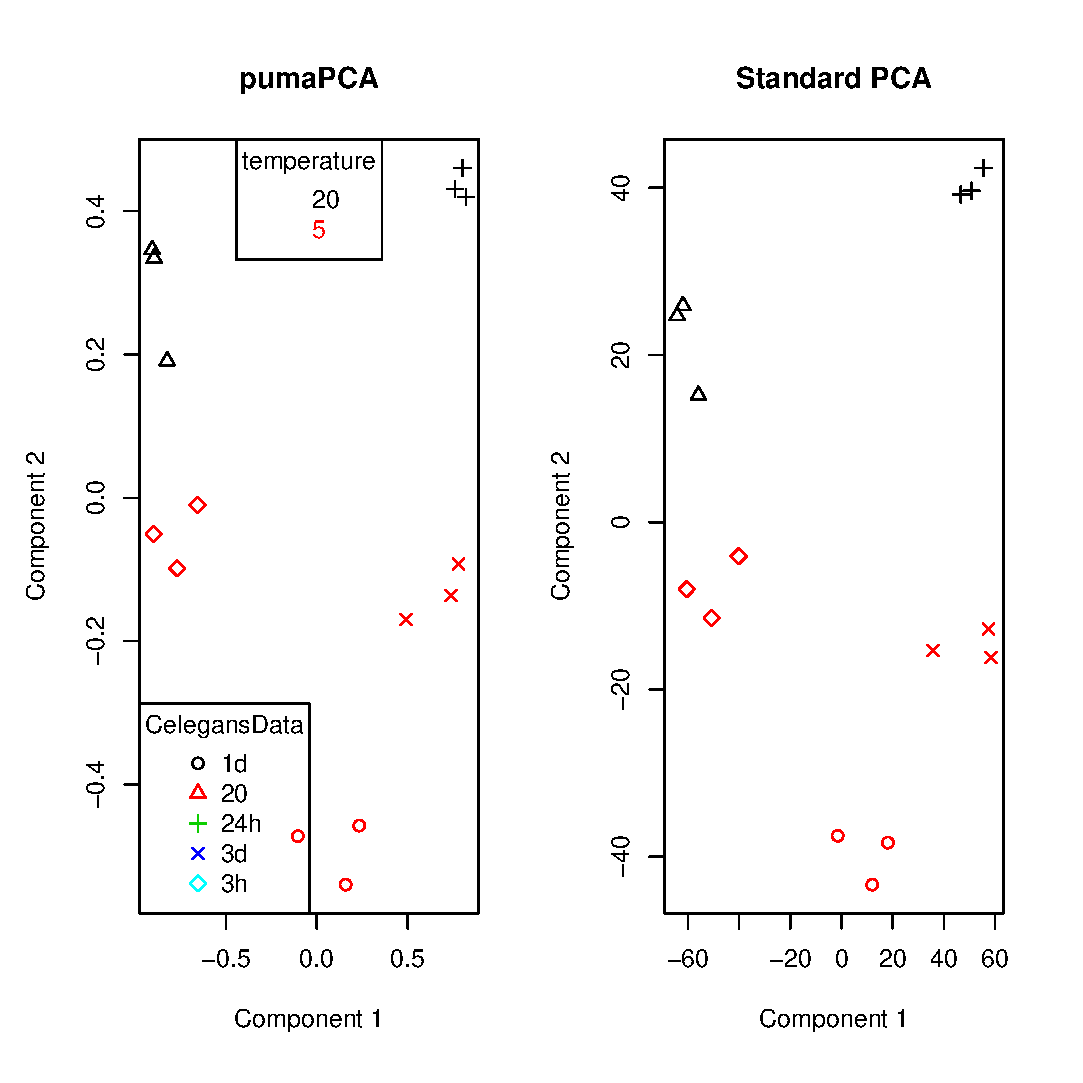
\includegraphics[width=0.7\textwidth,keepaspectratio]{PCA2.eps}
		\rule{35em}{0.5pt}
	\caption[Principal component analysis of time series data ]
		{Principal component analysis of gene expression time series data}
	\label{fig:PCA_time_series}
\end{figure}

\subsection{Transcription Factors}
From different data sources we found different number/list of transcription factors for \textit{C. elegans}. \cite{Inmaculada:2007} build a database named \textit{C. elegans} differential gene expression database (EDGEdb) which contains the sequence information about 934 predicted transcription factors and their DNA binding domains. Initially we took these 934 transcription factors for our baseline experimental setup but we also kept the opening to deal with any number of transcription factor depending on the requirement/ update of the sequence information of transcription factors.

\subsection{Connectivity Information}
Network motifs are the simplest units of transcriptional regulatory network's architecture. Particular regulatory mechanism such as positive and/or negative feedback loop can be well studied by these network motifs. Based on size and nature network motifs can grow in numbers and complexity. Autoregulation, multicomponent loop, single input, multiple inputs, feedforward, regulators chain are some of the simplest and well known network motifs. Figure:\ref{fig:networkMotif} shows their representation. \cite{Xie:2005} used motif conservation information for higher organisms like human, dog, rat and mouse. For promoter analysis they considered a number of network motif (also known as transcription factor binding sites) and also some new motifs. These type of data termed as connectivity data by \cite{Liao:2003} and provide information about whether a certain transcription factor can bind the promoter region of a gene or not.

\begin{figure}
	\centering
		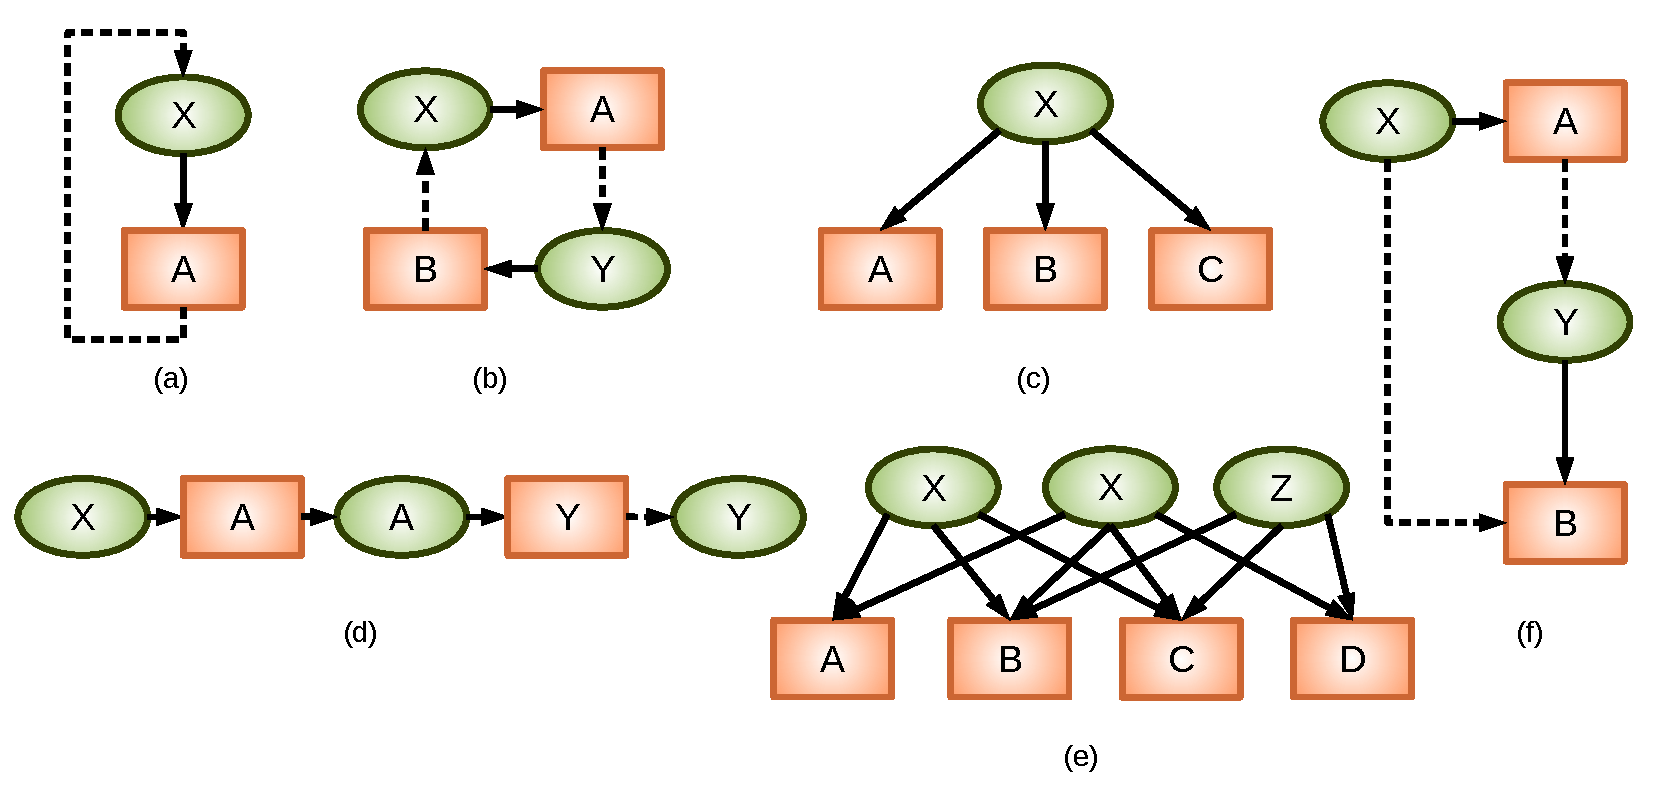
\includegraphics[width=0.95\textwidth,keepaspectratio]{NetworkMotif.pdf}
		\rule{35em}{0.5pt}
	\caption[Basic examples of network motif]
		{Some basic examples of network motif: (a). autoregulation, (b). multi-component loop, (c). single input motifs, (d). regulators chain, (e). multiple inputs, (f). feedforward motifs. Here green ovals represents regulators and orange rectangles represents gene promoters. Solid lines represent binding of a regulator to a promoter while dashed arrow represents gene encoding regulators binding their respective regulators.}
	\label{fig:networkMotif}
\end{figure}

\cite{WormNet} is a gene network of protein-encoding genes for \textit{C. elegans} based on probabilistic function and modified Bayesian integration. They have considered 15,139 genes and 999,367 linkages between genes associated with a log-likelihood score (LLS). These measured scores represents a true functional linkage between a pair of genes (\cite{Lee:2007}). The linkage between two genes were measured based on the following evidence codes-
\begin{itemize}
 \item CE-CC: 	Co-citation of worm gene
 \item CE-CX: 	Co-expression among worm genes
 \item CE-GN: 	Gene neighbourhoods of bacterial and archaeal orthologs of worm genes
 \item CE-GT: 	Worm genetic interactions
 \item CE-LC: 	Literature curated worm protein physical interactions
 \item CE-PG: 	Co-inheritance of bacterial and archaeal orthologs of worm genes
 \item CE-YH: 	High-throughput yeast 2-hybrid assays among worm genes
 \item DM-PI: 	Fly protein physical interactions
 \item HS-CC: 	Co-citation of human genes
 \item HS-CX: 	Co-expression among human genes
 \item HS-DC: 	Co-occurrence of domains among human proteins
 \item HS-LC: 	Literature curated human protein physical interactions
 \item HS-MS: 	human protein complexes from affinity purification/mass spectrometry
 \item HS-YH: 	High-throughput yeast 2-hybrid assays among human genes
 \item SC-CC: 	Co-citation of yeast genes
 \item SC-CX: 	Co-expression among yeast genes
 \item SC-DC: 	Co-occurrence of domains among yeast proteins
 \item SC-GT: 	Yeast genetic interactions
 \item SC-LC: 	Literature curated yeast protein physical interactions
 \item SC-MS: 	Yeast protein complexes from affinity purification/mass spectrometry
 \item SC-TS: 	Yeast protein interactions inferred from tertiary structures of complexes
\end{itemize}

We have constructed the connectivity matrix between genes and associated transcription factors from the gene to gene linkage and log-likelihood scores. We choose co-expression among worm genes (CE-CX), high-throughput yeast 2-hybrid assays among worm genes (CE-YH), literature curated human protein physical interactions (HS-LC) and high-throughput yeast 2-hybrid assays among human genes (HS-YH) to start our experiments. But if needed we can consider any of the evidence to reconstruct the connectivity matrix. From the gene list we have picked the protein-coding genes (i.e. transcription factors) and later 
binarized it. If there is an associated LLS value between a gene and a transcription factor we set the value '1' and '0' otherwise.

\section{Result Analysis}
We have developed a $R$ based tool $chipDyno$ for the identification of quantitative prediction of regulatory activities of the gene specific TFA through posterior estimation. The \textit{ChipDyno User Guide} \footnote{\textit{ChipDyno User Guide} is available at GitHub} explains different functionality of this tool and working pathway. There is no established benchmarks or baseline, nor a known ground truth to which to compare to our results of gene specific TFA for \textit{C. elegans}.

\begin{figure}
	\centering
		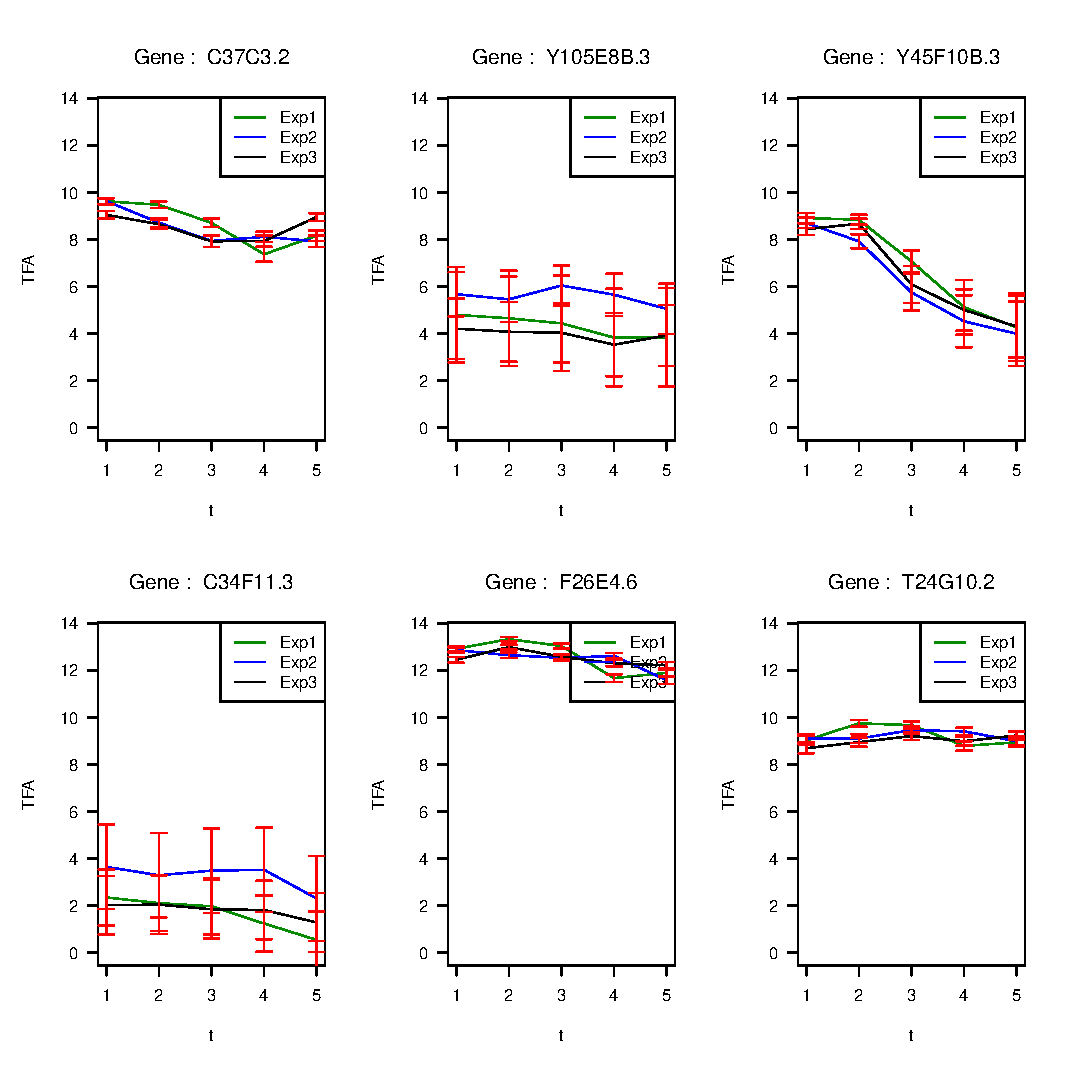
\includegraphics[width=\textwidth,keepaspectratio]{ZK370_2_3.eps}
		\rule{35em}{0.5pt}
	\caption[Gene Specific transcription factor activity of ZK370.2]
		{Gene Specific transcription factor activity of ZK370.2 on (top left to right) C37C3.2, Y105E8B.3, Y45F10B.3 and (bottom left to right) C34F11.3, F26E4.6, T24G10.2. $x$-axis represent the time stage of the experiments and $y$-axis represent the gene expression level for transcription factor activities. Three different line represent TFA for three replication and red vertical lines are error bars.}
	\label{fig:TFA_of_of_ZK370.2}
\end{figure}

According to \cite{WormNet} the number of gene of \textit{C. elegans} is 15,139 and \cite{Inmaculada:2007} presented 934 transcription factors. All the network motif, i.e. autoregulation, multi-component loop, feedforward loop, single input, multi-input motif, regulator chain were visible for transcription factor activity. So it was a mammoth task to choose all the transcription factors and show their activity. Rather we choose some random transcription factor and tried to find out its activity on different genes.

\begin{figure}
	\centering
		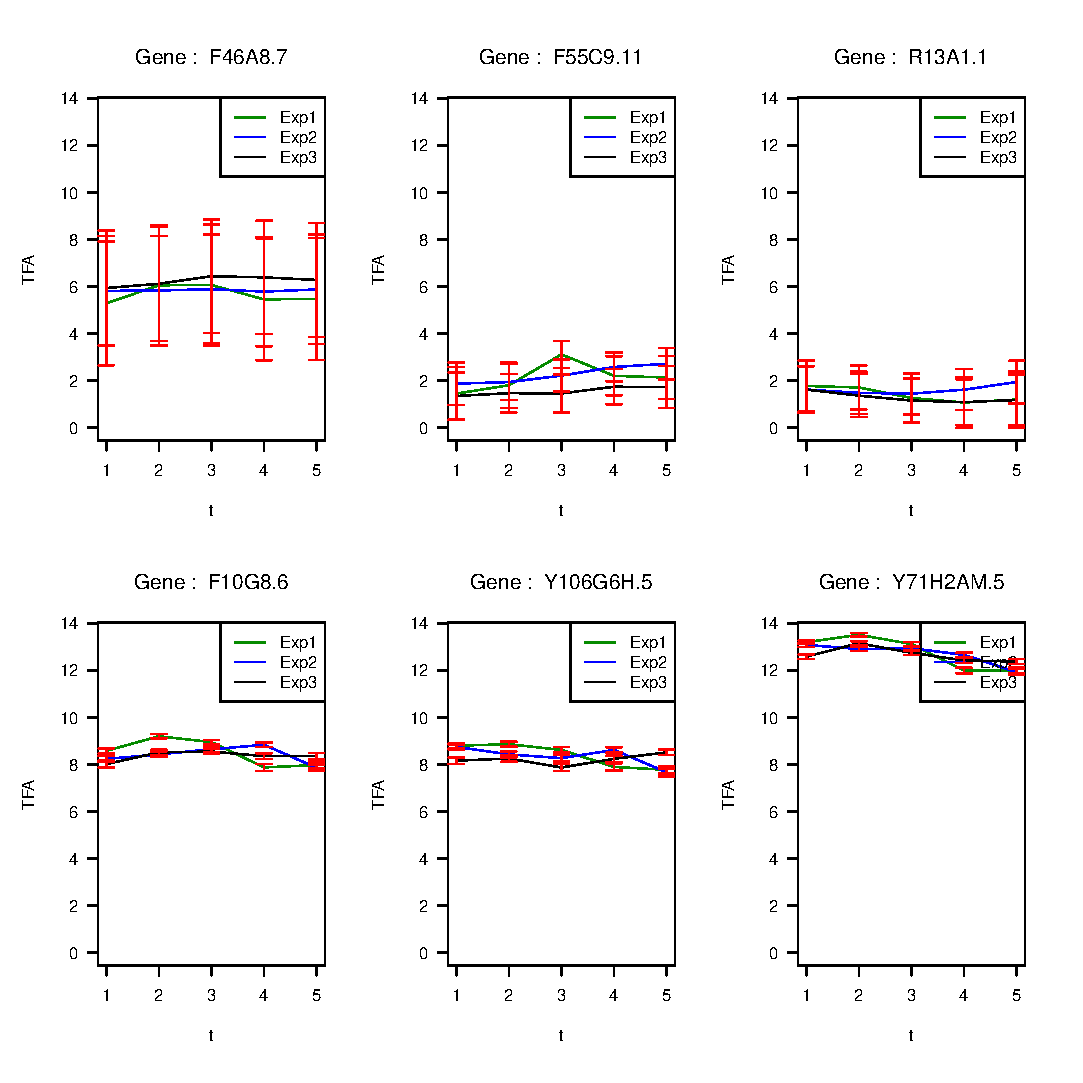
\includegraphics[width=\textwidth,keepaspectratio]{T20B12_8_3.eps}
		\rule{35em}{0.5pt}
	\caption[Gene Specific transcription factor activity of T20B12.8.3]
		{Gene Specific transcription factor activity of T20B12.8.3 on (top left to right) F46A8.7, F55C9.11, R13A1.1 (bottom left to right) F10G8.6, Y106G6H.5 and Y71H2AM.5. $x$-axis represent the time stage of the experiments and $y$-axis represent the gene expression level for transcription factor activities. Three different line represent TFA for three replication and red vertical lines are error bars.}
	\label{fig:TFA_of_of_T20B12_8_3}
\end{figure}

As a random sample we choose transcription factor ZK370.2 and find its activity on different genes. Figure \ref{fig:TFA_of_of_ZK370.2} shows that transcription factor ZK370.2 can regulate C37C3.2, Y105E8B.3, Y45F10B.3, C34F11.3, F26E4.6 and T24G10.2. In the dataset we had three replication of same experimental setup and its outcome. We performed our \textit{in-silico} experiments for individual replications and collected the results. Later we visualize all the outcome together by plots (some examples are Figure:\ref{fig:TFA_of_of_T20B12_8_3}, Figure:\ref{fig:TFA_of_of_ZK370.2}). From our experimental result we can say that the dynamics for some of the gene specific regulations (i.e. F26E4.6 and T24G10.2) are very flat and not that much informative but for some genes TFAs varies notably over time (i.e. C37C3.2 and Y45F10B.3). These are the genes which are regulated significantly by this transcription factor. For some cases (e.g\ gene C34F11.3) the error bar is quite high. These are the examples of bindings where there regulation is not that much significant or false positive could be an issue here. The magnitude of TFA also differs from one to another. We picked another random transcription factor T20B12.8.3. Figure \ref{fig:TFA_of_of_T20B12_8_3} shows its activity on different genes.

%TODO \subsection{PCA} ???

\subsection{Gene with multiple regulators}
For the case of multi input motif a single gene could be regulated by multiple transcription factors. Our developed tool can determine the posteriori of the relative weight for the different transcription
factors regulating the genes. Table \ref{table:Genes_regulated_by_multiple_TF} shows some examples. Gene C44B12.5 can be regulated by transcription factor Y116A8C.35 and F33A8.3. While gene
Y105E8B.3 is regulated by T20B12.8, F33A8.3, Y116A8C.35, F11A10.2 and C16A3.7. Though for some cases the expression level is quite low and noise margin is significantly high (examples of binding with insignificant regulation) but we can rank these genes using the ranking method of \cite{Kalaitzis:2011}.

\begin{table}
	\centering
\begin{tabular}{l l }
      \toprule
      \textbf{Gene Name} & \textbf{Regulators activity} \\
      \midrule
	      C44B12.5 & Y116A8C.35 = $ 1.719797 \pm 3.493205 $, \\ 
		       & F33A8.3 = $ 1.415785 \pm 3.492985$ \\~\\

	      Y105E8B.3 & Y54G2A.1 = $ 0.07157665 \pm 1.2222137 $ \\
			& F33D11.12 = $ 0.03861905 \pm 0.7252534 $ \\
			& ZK370.2 = $ -1.20157055 \pm  2.0318513 $\\~\\
		    
	      Y105E8B.3 & T20B12.8 = $ 0.25474933 \pm  2.5665869 $ \\
		  	& F33A8.3 = $ 0.11619828  \pm  3.5107742 $ \\
 		  	& Y116A8C.35 = $ 0.03289664 \pm  3.8071374 $ \\
			& F11A10.2 = $ 0.03016348 \pm 1.7737585 $ \\
 		  	& C16A3.7 = $ 0.01883489 \pm  0.9431105$\\
  \bottomrule
  \end{tabular}
	  \caption[Example of genes regulated by multiple TF]
		  {Example of genes regulated by multiple TF}
	  \label{table:Genes_regulated_by_multiple_TF}
\end{table}

\subsection{Different clusters and related active TF}
Clustering of genes is used to identify set of genes with similar behaviour (i.e.\ similar expression level or pattern) over a set of experiments (\cite{Eisen:1998}). Clusters provide an intuitive way to visualize the data and also help to facilitate the functional annotation of the not yet characterized genes. If an uncharacterised gene belongs to a cluster then the unknown gene could possibly have similar function and may dominated by genes of same function \cite{Pe'er:2003}. \cite{Cossins:2007} performed some cluster analysis of the genes based on different phenotype and its subsequent activities of the cell properties. They constructed the basic clusters with the following phenotype properties:

\begin{figure}
	\centering
		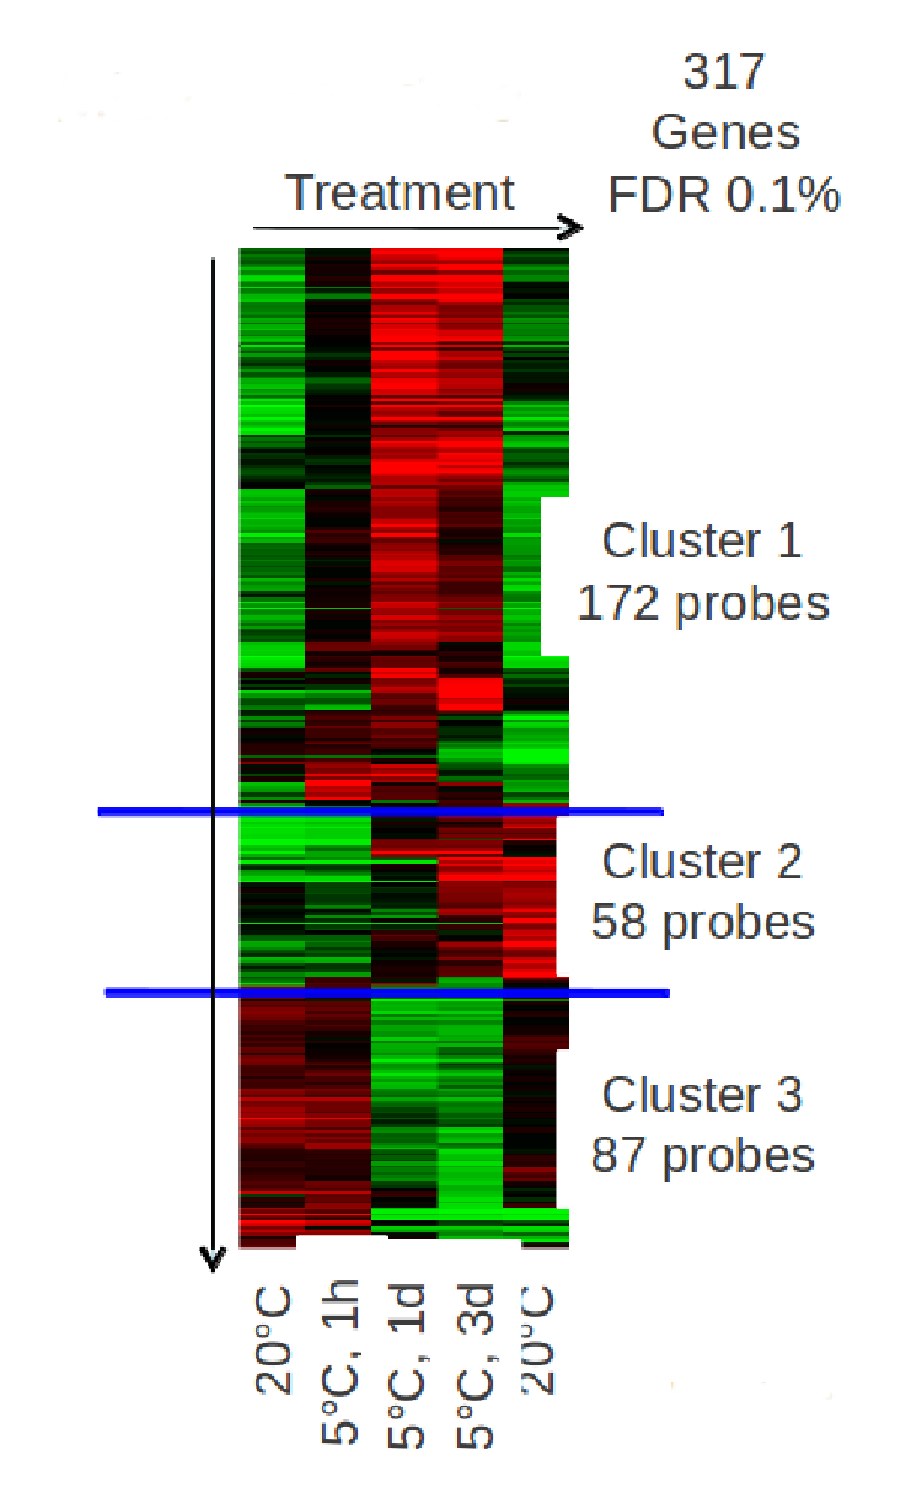
\includegraphics[scale=.5]{mcd3.eps}
		\rule{35em}{0.5pt}
	\caption[Clustering genes from microarray sample]
		{Clustering gene expression data from microarray sample: Each row corresponds to a single gene and each column corresponds to a microarray sample. This is an ordered representation of rows and columns.}
	\label{fig:Clustering_TF}
\end{figure}

\textbf{Cluster 1 - Chill upregulated} basically related with cell morphogenesis, cell growth, regulation of cell size, electron transport regulation of cell growth, generation of precursor metabolites and energy, anatomical structure morphogenesis, cellular metabolic process, proteolysis, etc.

\textbf{Cluster 2 - Chill late upregulated} related with chromosome organization and biogenesis, DNA packaging, chromatin architecture chromatin modification, negative regulation of developmental process, 
chromatin remodelling, regulation of developmental process, DNA metabolic process larval development (sensu Nematoda), organelle organization and biogenesis, post-embryonic development etc.

\textbf{Cluster 3 - Chill downregulated genes} related with amino acid and derivative metabolic process, carboxylic acid metabolic process, organic acid metabolic process, fatty acid metabolic process,
amino acid metabolic process, monocarboxylic acid metabolic process, etc.  Rest of the genes were placed in the group 'Others'. 

Figure \ref{fig:Clustering_TF} shows heat map generated from DNA microarray data to reflect the gene expression values at different temperature and their basic clusters \cite{Cossins:2007}. Based on the above clusters we also investigate about the transcription factors active in different clusters. Table \ref{table:Active_TF_diff_clusters} shows the numbers active transcription factor for each clusters.
For further analysis we can present the full list.

\begin{table}
  \centering
  \begin{tabular}{l l }
    \toprule
    \textbf{Clusters} & \textbf{Active TF} \\
    \midrule
    1. Chill upregulated & \bf 6 \\ 
    2. Chill late upregulated & \bf245 \\ 
    3. Chill downregulated & \bf128 \\
    4. Others & \bf 203 \\
  \bottomrule
  \end{tabular}
  \caption[Active TF on different clusters]
	  {Active TF on different clusters}
  \label{table:Active_TF_diff_clusters}
\end{table}

\section{Ranking Differentially expressed gene expressions}
\cite{Kalaitzis:2011} analysed the time series gene expression and filter the quiet or inactive genes from the differentially expressed genes. They have developed the model considering the temporal nature of data using Gaussian process. We have used this model to rank our time series gene expression and ranked the differentially expressed gene expressions. We ranked the three replicates of our data separately and later determine the Pearson correlation between ranking score of different samples.

\begin{figure}
	\centering
		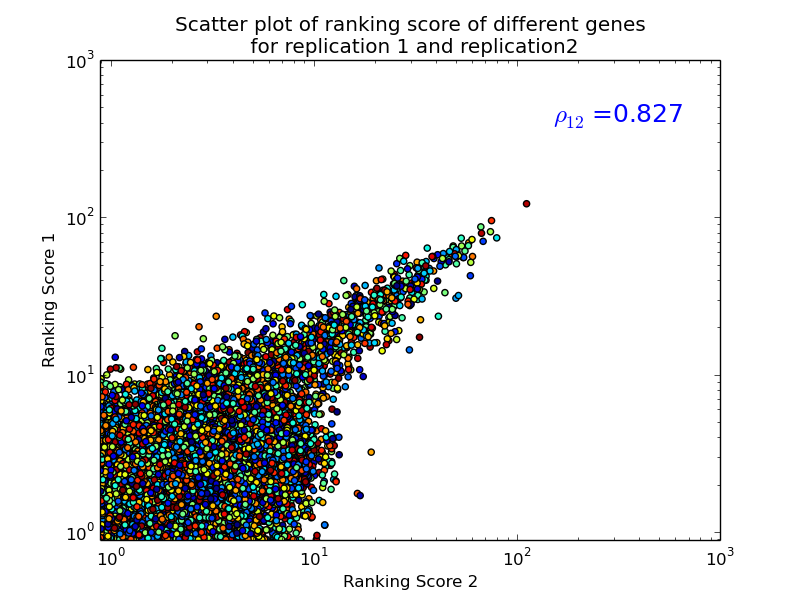
\includegraphics[width=0.63\textwidth,keepaspectratio]{rs12.png}
		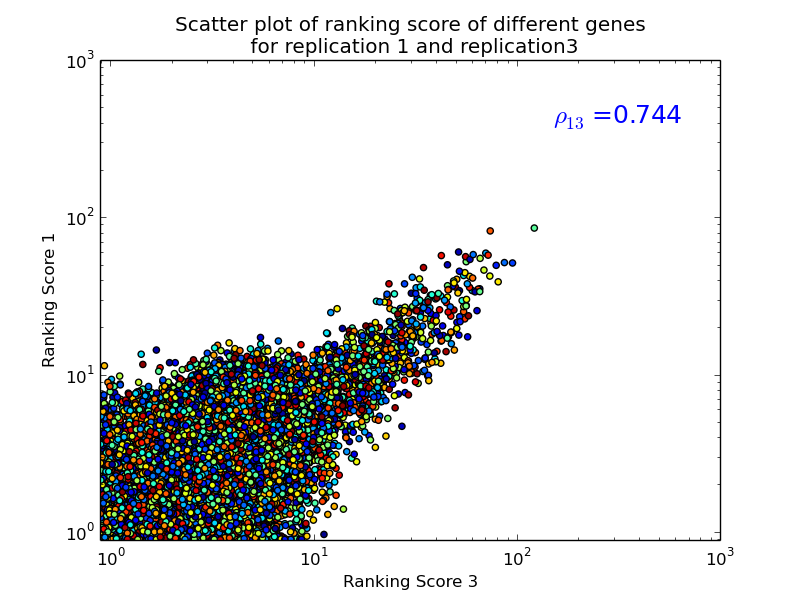
\includegraphics[width=0.63\textwidth,keepaspectratio]{rs13.png}
		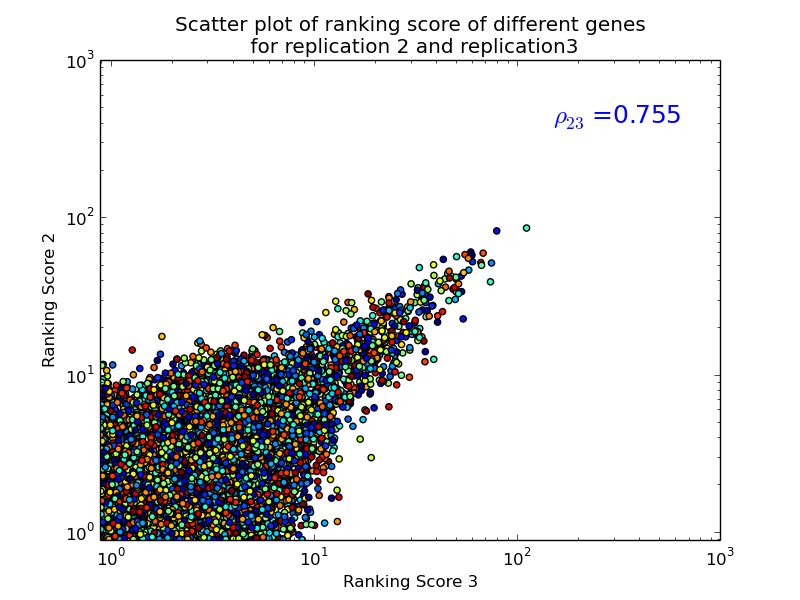
\includegraphics[width=0.63\textwidth,keepaspectratio]{rs23.png}
		\rule{35em}{0.5pt}
	\caption[Pearson's correlation between different ranking scores]
		{Pearson's correlation between different ranking scores. For each figure number at the top right position represent Pearson's correlation}
	\label{fig:ranking_scores}
\end{figure}

Figure \ref{fig:ranking_scores} shows the Pearson correlation between different ranking scores. The correlation coefficient for all three relations (between sample 1 and sample 2, sample 2 and sample 3 and
sample 3 and sample 1) were quite high. Which indicates the similarity of differentially expressed genes and quiet genes of different samples or replication of time series data. So, if required, based on these ranking we can easily filter out some of the quiet genes and keep the other genes for further experiments.

\section{Discussion}
%TODO

%\section{Convetional Approach of Clustering and related TFs}

% %TODO
% 
% http://tex.stackexchange.com/questions/132526/overbrace-with-square-bracket
% \[
%  \overbrace{a+b+c}^{d} \quad \aoverbrace[L1R]{a+b+c}^{d} \quad
%  \underbrace{a+b+c}_{d} \quad \aunderbrace[l1r]{a+b+c}_{d}
% \]
%
% \section{Different models of TFAs}